% !TeX spellcheck = en_US
% !TeX encoding = UTF-8
%%%%%%%%%%%%%%%%%%%%%%%%%%%%%%%%%%%%%%%%%%%%%%%%%%%%%%%%%%%%
\chapter{Stress Detection Methodology}

 \autoref{fig:netwrokyt} outlines the whole process from collection of data to the classification of stress.


\begin{figure}[!htbp]
	\centering
	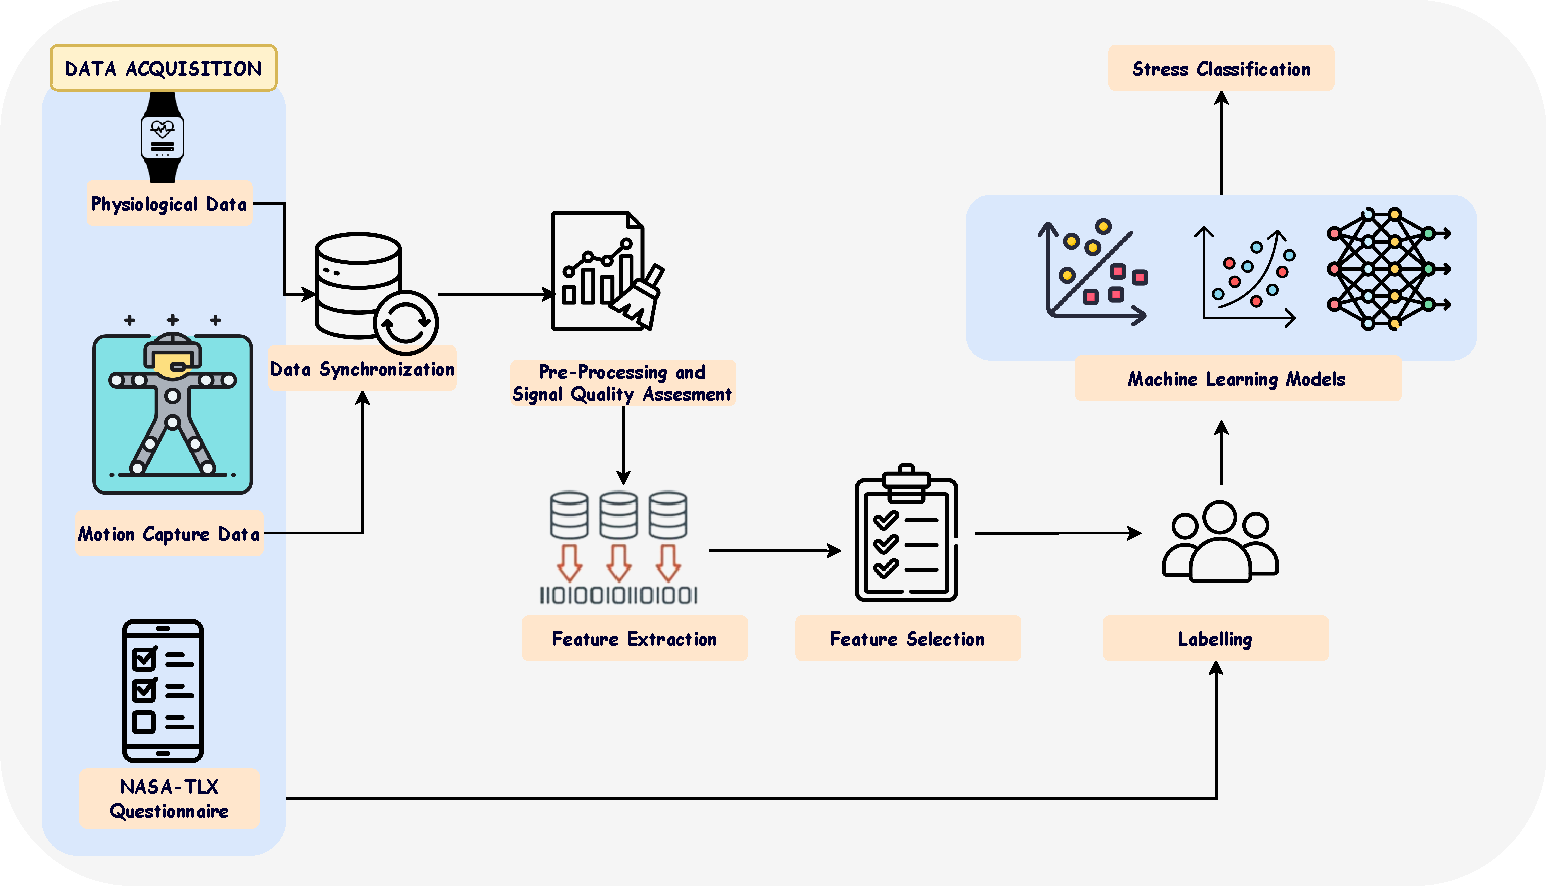
\includegraphics[width=\columnwidth]{images/schematic.pdf}
	\caption{Schematic of the experiment setup}
	\label{fig:netwrokyt}
\end{figure}

\section{Data Synchronization \gls*{gptmo}} \label{sec:synchronization} 
As previously eluded in section \ref{sec:expprot}, data synchronization is crucial to our experimental framework, ensuring the consistency
of data gathered from all the different sensors. In our setup, the Empatica E4 wristband collects various physiological signals, such as the BVP, EDA, HR, and ST at different frequencies, as well as the motion capture system that tracks the participant's movements at a higher frequency. Given the varying sampling rates of these data sources, it's crucial to synchronise them to ensure they are comparable and accurate.

The Empatica E4 samples the Blood Volume Pulse (BVP) data at a rate of 64Hz. However, it transmits other metrics like EDA and temperature at a lower rate of 4Hz. On the other hand, the Motive software captures the motion capture data at a higher rate of 120Hz. These differences in sampling rates require a careful synchronization approach.

Our synchronization strategy focuses on aligning all the different data streams to uniform and matching frequency. Considering the need for detailed data where we retain most of the information required, we standardise all data streams to a frequency of 64Hz, matching the Blood Volume Pulse (BVP) rate from the Empatica E4. This standardisation process involves downsampling the motion capture data, originally recorded at a higher frequency of 120Hz. Simultaneously, for other signals like the Electrodermal Activity (EDA) and temperature, updating at a lower frequency of 4Hz, and acceleration data at 32Hz, we use a forward-filling approach, carrying their most recent values until an update occurs.

A ROS node executes this synchronization. By using the BVP rate as the master reference, the node ensures that both physiological and motion data are synchronised in time. This alignment is critical for an integrated and comprehensive analysis of the participant's responses, providing a dataset that accurately reflects both the physiological states and motion data.

Once synchronised, the data is then published to a ROS topic, typically \textit{/aggregated\_data}. This topic carries a comprehensive stream of information that combines detailed physiological measures with motion data. This dataset forms the foundation for subsequent analysis phases in our study, such as feature extraction and stress detection.

\section{Pre-Processing \gls*{gptmo}} 
Pre-processing is a crucial step in analysing data from physiological sensors and motion capture systems, as it prepares the raw data for subsequent processing and analysis phases.The pre-processing and subsequent feature extraction were done using the BIOBSS library in python\parencite{biobss}. This section outlines the key aspects of pre-processing in our study.

\subsection*{Data Filtering} \label{sec:data_filtering}

In the pre-processing phase of our study, data filtering plays a crucial role in refining the quality of the signals gathered from the physiological sensors and motion capture systems. This step involves applying specific filtering techniques to the raw data to remove unwanted data, thereby enhancing the signal's clarity and usability for further analysis.

The primary objective of data filtering is to isolate the significant aspects of the signal while eliminating any unwanted noise or interference. Different filtering methods are employed depending on the nature of the signal and the type of noise present. For instance, we use N-th-order Butterworth filters, which effectively retain the desired frequency range while attenuating frequencies outside this range. The Butterworth filter is known for its smooth frequency response and is particularly useful in physiological signal processing, where preserving the signal's integrity is crucial.

Each signal type dictates specific filter parameters like filter order, cutoff frequencies, and filter type (lowpass, highpass, or bandpass). This careful selection ensures that the final signal is representative of the true physiological data crucial for accurate analysis.

\subsection*{Data Normalisation }
Normalisation is a critical step in data pre-processing as well, particularly when dealing with signals of varying magnitudes or scales. Our approach involves applying a normalisation process to each input signal, standardising the data values range. This step is essential for comparing and combining data from different sensors effectively.

The method we use for normalisation is primarily the 'z-score' method. This technique transforms the data into a mean of zero and a standard deviation of one. Doing so ensures that each signal contributes equally to the analysis, irrespective of their original scale or distribution. This standardisation is crucial for machine learning models, as it enhances algorithm performance and prevents any single feature from dominating due to its scale.

Normalisation also aids in mitigating the impact of outliers, as it brings all data points onto a common scale, making them more suitable for analysis.

\begin{comment}
\subsection*{Peak Detection }
Peak detection is a method used to identify significant local maxima (peaks) and minima (troughs) in the data, which can represent important events or changes. In the context of stress detection, for instance, identifying peaks in heart rate or GSR signals can be indicative of moments of heightened stress or arousal. Efficient peak detection algorithms are crucial for accurately identifying these critical points in the data. Analyzing the frequency and intensity of these peaks can provide valuable insights into the physiological response patterns of the participants, such as the frequency of stress episodes or the degree of response to different stimuli.
\end{comment}

\subsection*{Signal Quality Assessment }
\label{sec:signal_quality_assessment }

Signal quality assessment is an integral part of the preprocessing phase to ensure the reliability and accuracy of data collected from sensors, which is fundamental for accurate analysis. Various methods are employed to assess the quality of signals, each targeting specific types of anomalies or artefacts.


\paragraph{Detection of Clipped Segments:}
This method involves identifying segments in the signal that are clipped or truncated. Clipping often occurs when the signal amplitude reaches the sensor's recording capacity limits. By setting thresholds for positive and negative clipping, the method detects and marks these segments, facilitating their exclusion or correction.

\paragraph{Detection of Flatline Segments:}
This method identifies flatline segments where the signal shows minimal variation over a period. Such segments can indicate sensor displacement or malfunction. The method identifies these periods by assessing the duration of flatness and the threshold for change in signal amplitude, helping exclude non-physiological data from the analysis.


Each method plays a crucial role in verifying the integrity of the signal data. Identifying and addressing issues like clipping, flat-lining, and inconsistent patterns, signal quality assessment ensures that subsequent data analysis stages are based on accurate and reliable data. Among our 20 participants, 5 participants experienced  flat-lining indicating that the data had not been collected properly, so they were excluded from further analysis.



\subsection*{Baseline Correction}
\label{sec:baseline_correction}

Baseline correction forms a pivotal part of our data normalisation strategy, particularly tailored for participant-specific physiological data. This approach is centered around the concept of adjusting the data relative to each participant's baseline physiological state, captured during a rest period prior to the experimental tasks. This preparatory measure establishes a reference point against which subsequent physiological responses are compared.
In the baseline correction process, we begin by computing the average values of physiological signals recorded during the baseline phase before the start of the experiment. This baseline phase is critical as it represents a period of rest where the participant's physiological state is unaffected by experimental stressors. By establishing this baseline, we are able to set a reference point that reflects the participant's normal physiological state. Subsequently, we adjust the data points collected during the active phases of the experiment relative to these baseline averages. This adjustment is a normalisation process that centers the data around a personalised zero point, effectively accounting for individual physiological variations. The core advantage of baseline correction lies in its ability to mitigate the influence of inter-individual variability on the physiological measurements. Since each participant exhibits unique baseline characteristics and responds differently to stressors and other factors, the process of normalizing data against individual baselines serves as a valuable means to address this variability and achieve a more accurate and personalised assessment of stress responses.

This method ensures that the changes observed in the physiological data during the experiment are indicative of the participant's response to the experimental conditions rather than being a reflection of their baseline physiological state.

\subsection*{Signal Segmentation}
\label{sec:signal_segmentation}
In our research, the segmentation of physiological data into windows was a crucial part of the preprocessing. This process involved breaking down the continuous data streams into smaller, manageable sliding windows for detailed analysis. The selection of window size and step size was critical and was tailored based on the characteristics of the signal and the objectives of our analysis.

The window size was carefully chosen to capture relevant physiological and behavioral patterns within each segment, balancing the need to encapsulate meaningful data against the computational demands of processing. The step size determined the overlap between these windows, ensuring continuity and that no significant transient events were missed.

Accounting for the sampling rate of each signal was vital in customizing the segmentation process appropriately. This flexible approach was key to accommodating different types of signals, ensuring that the window size was appropriate for the length of the signal and that the segmentation parameters were compatible with each signal's nature.

Segmenting data into Windows enabled us to convert the ongoing data streams into a format suitable for comprehensive analysis. This structured approach facilitated subsequent computational processes, including feature extraction and pattern recognition, essential for robust stress detection and analysis.

\section{Feature Extraction \gls*{gptmo}}
Feature extraction and selection play a pivotal role in the effectiveness of machine learning models, especially in the context of human stress recognition. Feature extraction involves deriving meaningful attributes from the raw data collected. The features extracted can vary widely, including statistical features, time-domain, frequency-domain, and linear and non-linear features.

The complexity of these features can range from basic statistical measures like mean, median, minimum, and maximum to more intricate features based on specific data modalities. Each used in stress detection may yield a unique set of features, contributing to the overall data analysis and model accuracy. The selection and application of these features are crucial, as they directly impact the classification stage, ultimately influencing the model's performance in stress recognition.

Comprehensive reviews have been conducted on this, notable \textcite{review1}, \textcite{arsalan}. We have utilised these extensive analyses as a foundation to select and identify the appropriate features into our study.


\subsection{Blood Volume Pulse}
Photoplethysmography (PPG) sensors provide a non-invasive optical method to acquire Blood Volume Pulse (BVP) signals, detecting volumetric blood flow changes as explained \autoref*{subsec:PPGtheory}. Among the various metrics that can be extracted from PPG signals, gls{HR} and  gls{HRV} are prominent. These features offer critical insights into cardiac function and stress response. Detailed discussion of HR and HRV feature extraction from PPG will follow later.

After initial pre-processing of the PPG signal, which includes filtering, baseline correction, normalisation, and signal quality assessment, the pivotal step in signal analysis is peak detection. This involves accurately identifying systolic peaks in the blood volume pulse, crucial for calculating HR and HRV aswell.

The PPG waveform typically comprises two peaks: systolic and diastolic. While systolic peaks are usually prominent, diastolic peaks may not be observable in certain conditions. However, when identifiable, diastolic peaks offer additional information, contributing to a more comprehensive analysis.

To locate the diastolic peak, analysis often involves examining the first and second derivatives of the PPG signal, known as the  gls{VPG} and  gls{APG}, respectively \parencite{apg}. Identifying fiducial points on VPG and APG is critical, as these points can provide insights into blood pressure estimation and other advanced cardiovascular analyses.

PPG signal analysis encompasses a variety of features across different domains:

\paragraph*{Time Domain/Morphological Features}: These features are directly extracted from the morphology (shape and structure) of the PPG waveform.
These include cycle duration, peak amplitudes, and ratios of different waveform components. These features give insights into the blood volume changes with each heartbeat and can indicate changes in peripheral blood flow dynamics.
\paragraph*{Frequency Domain Features}: Analysis of the frequency components of the PPG/BVP signals reveals the rhythmic patterns linked to cardiovascular dynamics. This typically involves power spectrum analysis to identify dominant frequencies.
\paragraph*{Statistical Features}: The statistical analysis of PPG/BVP signals includes calculating mean, standard deviation, skewness, and kurtosis, offering a comprehensive statistical overview of the waveform.
Advanced Feature Extraction through VPG and APG Analysis further deepens the understanding of cardiovascular dynamics. These derivatives of the PPG signal expose intricate details about blood flow, particularly regarding systolic and diastolic activities. Features derived from VPG and APG include amplitudes and durations of specific waves and ratios comparing different waveform components.

\subsection*{HR Features}
Heart Rate (HR) is a fundamental measure in cardiovascular and stress-related studies, representing the frequency of the heartbeat.It is considered to be the most widely adopted and straightforward measure to estimate stress levels \parencite{review1} It is typically expressed in beats per minute (bpm). The primary method of deriving HR from PPG involves counting the number of systolic peaks within a specified time frame.

Key features and analysis in HR:
\begin{itemize}
  \item \textbf{Mean and Standard Deviation of the R-R Interval:} Provide a basic understanding of heart rate variability. The mean R-R interval offers insight into average heart rate, while the standard deviation reflects the variability around this mean.
  
  \item \textbf{Root Mean Square of the Successive Differences (RMSSD):} Measures the short-term variability in R-R intervals, primarily reflecting parasympathetic nervous system activity.
  
  \item \textbf{Mean R Peak Amplitude:} The average amplitude of the R peaks in the PPG signal, indicating the strength and consistency of heartbeats.
  
  \item \textbf{Skewness and Kurtosis of R-R Intervals:} Statistical measures describing the distribution of R-R intervals. Skewness indicates asymmetry, while kurtosis indicates the 'tailedness' of the distribution.
  
  \item \textbf{Percentile of R-R Intervals:} Involves calculating specific percentiles (e.g., 50th, 95th) of the R-R interval distribution, providing additional insights into heart rate variability.
\end{itemize}



\subsection*{HRV Features}
Heart Rate Variability (HRV) analysis, an essential aspect of cardiac function understanding, is also derivable from PPG signals. HRV refers to the variation in the time interval between heartbeats, indicated by the beat-to-beat (R-R) intervals variation. It extends beyond a mere measure of cardiac rhythm, serving as an indicator of physiological resilience and adaptability in response to stress. HRV features extracted from PPG, including R-R interval and the root mean square difference of consecutive R-R intervals, are instrumental in assessing both heart rate dynamics and autonomic nervous system regulation.

Some of the key features in HRV analysis include:
\paragraph*{Time-Domain Features}
\begin{itemize}
    \item \textbf{SDNN (Standard Deviation of NN intervals):} Measures overall heart rate variability.
    \item \textbf{RMSSD (Root Mean Square of Successive Differences):} Reflects the beat-to-beat variance in heart rate and is particularly sensitive to changes in the parasympathetic nervous system.
    \item \textbf{NN50 and pNN50:} NN50 counts the number of pairs of successive NN intervals differing by more than 50 ms, and pNN50 is the proportion of NN50 to the total number of NN intervals.
\end{itemize}

\paragraph*{Frequency-Domain Features}
\begin{itemize}
    \item \textbf{Low Frequency (LF):} Represents a blend of sympathetic and parasympathetic activity.
    \item \textbf{High Frequency (HF):} Primarily reflects parasympathetic activity.
    \item \textbf{LF/HF Ratio:} Used to assess the balance between sympathetic and parasympathetic nervous systems.
\end{itemize}

\paragraph*{Non-Linear Features}
\begin{itemize}
    \item \textbf{SD1/SD2 (Poincaré Plot Analysis):} Provides a geometric representation of HRV, offering insights into the complexity of heart rate dynamics.
    \item \textbf{Sample Entropy:} Measures the complexity or irregularity of R-R interval time series.
\end{itemize}


\subsection{Electrodermal Activity \gls{gptmg}}

Electrodermal Activity (EDA), also known as galvanic skin response (GSR), is an indicator of emotional and physiological arousal, primarily influenced by the Sympathetic Nervous System (SNS). It primarily consists of two components: tonic (Skin Conductance Level, SCL) and phasic (Skin Conductance Response, SCR).As already explained in Section \ref*{subsec:EDAtheory} the tonic component represents baseline levels of skin conductance, reflecting slow changes in arousal state. The phasic component, on the other hand, captures rapid fluctuations in response to specific stimuli or events. \textcite{electrodermal}.

After the usual process of filtering, baseline correction and normalizing the signal as well as checking the quality of the signal we first decompose the EDA signal into its tonic and phasic components using continuous decomposition analysis. This process allows us to separately analyze the steady-state (SCL) and transient (SCR) aspects of skin conductance.
The decomposition is typically carried out either using a highpass or bandpass filtering techniques or a convex optimization algorithm cvxEDA \parencite{cvxEDA} , ensuring that each component accurately represents the underlying physiological processes.\autoref*{fig:eda sig} shows the decomposition of the EDA signal into its tonic and phasic components from the raw EDA signal.

\begin{figure}[!htbp]
	\centering
	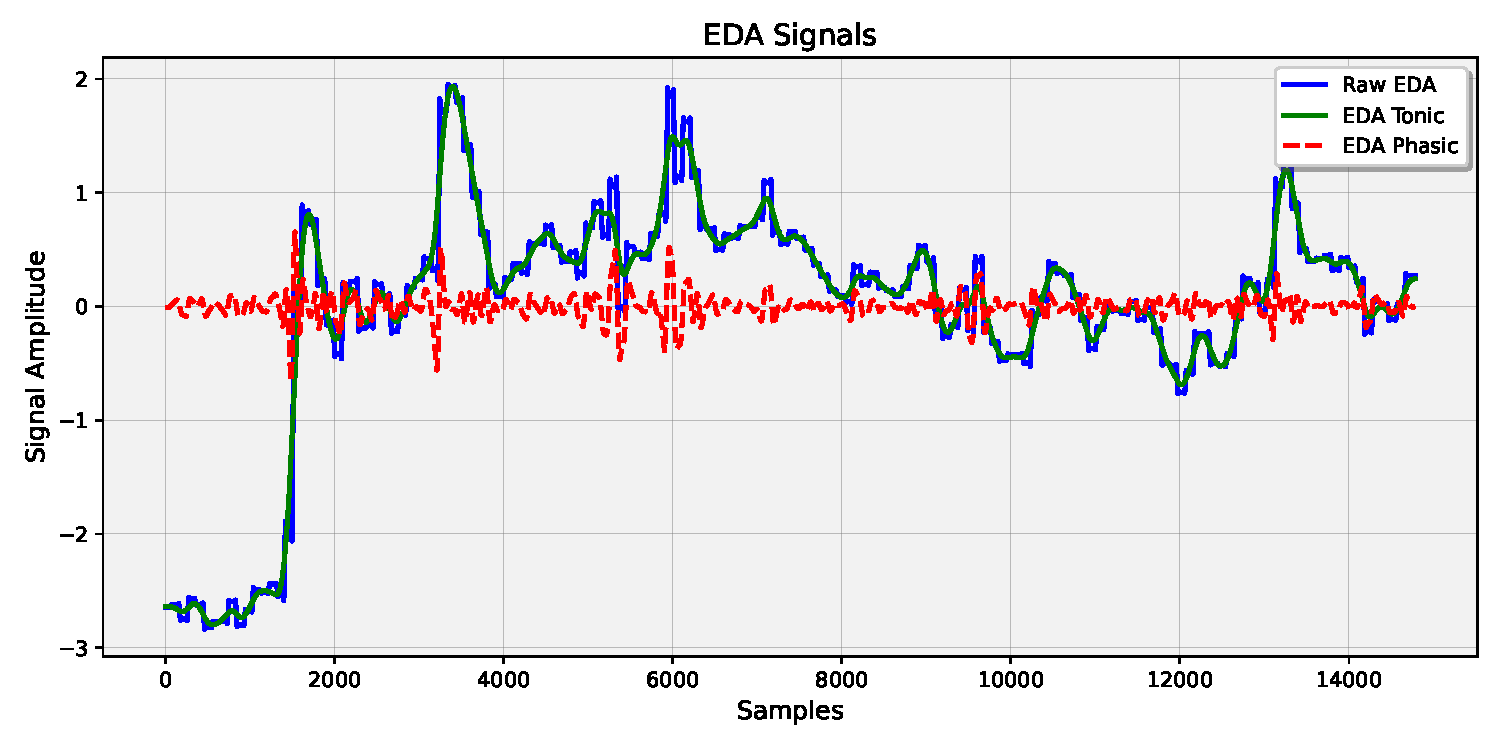
\includegraphics[width=\columnwidth]{images/edaplot.pdf}
	\caption{Phasic and tonic components of the EDA signal.}
	\label{fig:eda sig}
\end{figure}

The activity of sweat glands, predominantly controlled by the SNS, leads to an increase in SCR during emotional arousal \parencite{electrodermal}. Notably, the non-specific SCR (NS.SCR) is intricately related to cognitive processes and psychophysiological states, acting as a direct measure of arousal \parencite{177}. Unlike other physiological measures influenced by both sympathetic and parasympathetic nervous systems, SCR is exclusively modulated by the sympathetic nervous system, making it a reliable stress indicator \parencite{7}. Under stress, both the tonic (SCL) and phasic (SCR) components escalate due to increased skin moisture.

A thorough review and comparative analysis of various Electrodermal Activity (EDA) features have been conducted, as detailed by \textcite{EDAFeatures}. This process involved a meticulous examination of close to 40 distinct EDA features previously identified in the literature. The outcome of this comprehensive analysis guided us in carefully selecting the features most necessary to the objectives of our research.
Some of the key features from EDA include:

A detailed examination of the phasic component involves analyzing peak amplitude, frequency, and their inter-relationships in SCRs. This analysis is crucial for deciphering emotional and cognitive stress responses, as these metrics directly reflect the intensity and frequency of physiological reactions to stimuli.

From the decomposed EDA data, a variety of time domain statistical features can be extracted. These include mean ($\mu$), standard deviation ($\sigma$), coefficient of variance (CV), variance ($\sigma^2$), and kurtosis ($\beta$) from the phasic component.

Mean ($\mu$) provides a measure of the central tendency of the SCR amplitudes.
Standard deviation ($\sigma$) and variance ($\sigma^2$) capture the variability or dispersion around the mean.
The coefficient of variance (CV) offers a normalised measure of dispersion relative to the mean.
Kurtosis ($\beta$) evaluates the peakedness or flatness of the distribution of SCR amplitudes.

In addition to time-domain features, we analyze the EDA signal in the frequency domain. Furthermore, frequency-domain features like spectral power in specific bands (f1sc, f2sc, f3sc) and the overall energy and entropy of the signal gave us a spectrum-based view of the EDA responses. By analyzing these features, we could discern patterns and rhythms in the EDA that are not immediately apparent in the time-domain.


Detecting and analyzing peaks in the phasic component (SCRs) is crucial. Peak amplitude, frequency, and their inter-relationships can be strong indicators of emotional and cognitive stress responses.

By examining both tonic and phasic components, we can understand the sustained arousal level (SCL) and the specific responses to stimuli (SCR). The correlation between these components can provide valuable insights into how sustained stress levels influence responses to immediate stimuli.
From the tonic component, which encapsulates the underlying level of arousal, we calculated the mean, capturing the central tendency over time, and the standard deviation, offering insights into the variability around this mean. The maximum and minimum values, along with the range, provided us with the extremes of the EDA signal, painting a picture of the breadth of responses.

From the phasic component, we focused on the Skin Conductance Responses (SCRs) to discern more rapid changes associated with specific stimuli. We extracted features like SCR amplitude, which reflects the intensity of the response, and the frequency of these SCRs, indicating how often these responses occur. The kurtosis of SCR amplitudes, a measure of the 'tailedness' of the distribution, gave us an understanding of how peaked or flat the distribution of responses was, while the skewness indicated any asymmetry, offering clues about the predominant direction of the response distribution.

We also looked at the root mean square (RMS ), which is a measure of the signal's magnitude, providing a summative measure of the signal's complexity over a given period. The integral of the SCR signal (SCR Integral) was calculated to understand the total magnitude of these phasic responses over time. These features, alongside others like SCR momentum, which is akin to the second moment of the distribution, provided a comprehensive statistical breakdown of the phasic EDA signals.

\begin{comment}
\begin{table}[h]
  \centering
  \resizebox{\textwidth}{!}{%
  \begin{tabular}{|l|p{4cm}|l|l|l|}
  \hline
  \textbf{Feature}         & \textbf{Full Name}                                         & \textbf{Extracted From} & \textbf{Domain} & \textbf{Expected Behavior Under Stress} \\ \hline
  HR                       & Heart Rate                                                 & PPG-HR                 & Time Domain     & Increase                                \\ \hline
  MEAN IBI                 & Mean Interbeat Interval                                    & PPG-HRV                & Time Domain     & Decrease                                \\ \hline
  SDNN                     & Standard Deviation of NN intervals                         & PPG-HRV                & Time Domain     & Decrease                                \\ \hline
  RMSSD                    & Root Mean Square of Successive Differences                 & PPG-HRV                & Time Domain     & Decrease                                \\ \hline
  pNN50                    & Proportion of NN50 divided by total number of NNs          & PPG-HRV                & Time Domain     & Decrease                                \\ \hline
  Total Power              & Total Power of HRV spectrum                                & PPG-HRV                & Frequency Domain & Increase                                \\ \hline
  LF                       & Low Frequency                                              & PPG-HRV                & Frequency Domain & Increase                                \\ \hline
  HF                       & High Frequency                                             & PPG-HRV                & Frequency Domain & Decrease                                \\ \hline
  LF/HF                    & Low Frequency/High Frequency ratio                         & PPG-HRV                & Frequency Domain & Increase                                \\ \hline
  SD1                      & Poincaré Plot Standard Deviation perpendicular to the line of identity     & PPG-HRV & Non-Linear Domain & Varies                     \\ \hline
  SD2                      & Poincaré Plot Standard Deviation along the line of identity                & PPG-HRV & Non-Linear Domain & Varies                     \\ \hline
  SCL                      & Skin Conductance Level                                     & EDA                    & Time Domain     & Increase                                \\ \hline
  SCPh                     & Phasic Skin Conductance Signal Power                       & EDA                    & Frequency Domain & Increase                                \\ \hline
  SCRR                     & Number of Skin Conductance Responses                       & EDA                    & Frequency Domain & Increase                                \\ \hline
  SCdiff2                  & Skin Conductance Level Deviation Squared                   & EDA                    & Time Domain     & Increase                                \\ \hline
  EDA Level                & General Electrodermal Activity Level                       & EDA                    & Time Domain     & Increase                                \\ \hline
  Peak Amplitude           & Maximum Amplitude of Skin Conductance Response             & EDA                    & Time Domain     & Increase                                \\ \hline
  Rise Time to Peak        & Time to Reach Peak Amplitude from Onset                    & EDA                    & Time Domain     & Decrease/Varies                         \\ \hline
  Decay Time               & Time to Decrease from Peak Amplitude to Baseline           & EDA                    & Time Domain     & Increase/Varies                         \\ \hline
  Half Recovery Time       & Time for SCR Amplitude to Reduce to Half                   & EDA                    & Time Domain     & Increase/Varies                         \\ \hline
  Response Latency         & Time between Stimulus Onset and Start of SCR               & EDA                    & Time Domain     & Increase/Varies                         \\ \hline
  EDR Rate                 & Event-Related SCR Rate                                     & EDA                    & Frequency Domain & Increase                                \\ \hline
  \end{tabular}}
  \caption{Physiological Markers for Stress Detection in PPG and EDA Signals}
  \label{tab:stress_markers}
\end{table}
\end{comment}


\subsection{Body Features \gls{gptmo}}
Since we captured human motion using the motion capture system, we selected 13 key points from the 25 marker points used by the system, focusing on the upper body. The chosen points were Hip, Abdomen, Chest, Neck, Head, Left Shoulder (LShoulder), Left Upper Arm (LUArm), Left Forearm (LFArm), Left Hand (LHand), Right Shoulder (RShoulder), Right Upper Arm (RUArm), Right Forearm (RFArm), and Right Hand (RHand). These points were strategically selected to comprehensively capture the whole upper body movements. The arrangement of these points is depicted in \autoref{fig:human1}



\begin{figure}[!htbp]
	\centering
	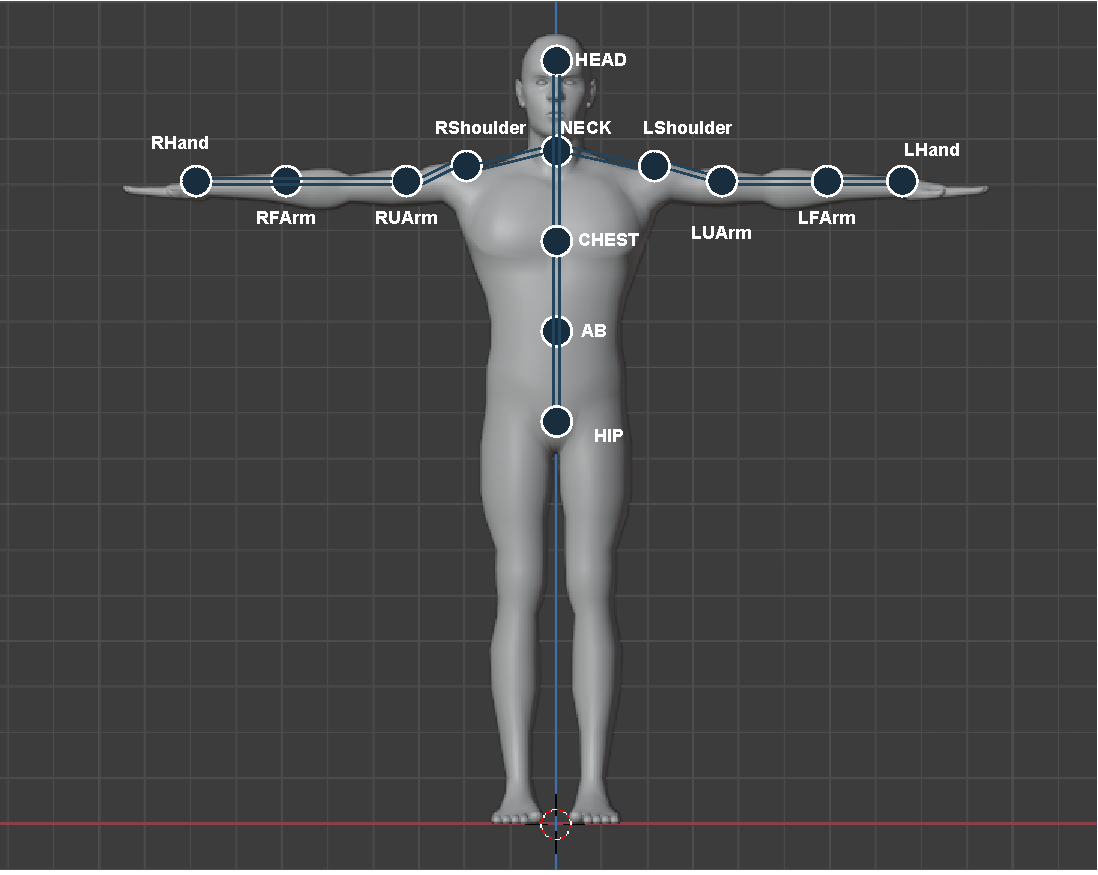
\includegraphics[width=0.8\columnwidth]{images/humandraw.pdf}
	\caption{13 points from the motion capture} 
	\label{fig:human1}
\end{figure}
%\textcite[postnote]{HARRIGAN19851161} HARRIGAN19851161
\subsection*{Self Touching} 
\textcite{10.1371/journal.pone.0043571} has shown that body posture and body language can be valuable indicators of stress. In line with this, we also explored body language cues such as self-touching, which \textcite{HARRIGAN19851161} suggests can be indicative of negative affect, such as anxiety or discomfort. Specifically, we focused on face and head touching as potential stress indicators.

To determine whether an individual is touching their face, the distances between their hand and head, and between their hand and neck, are measured. When either of these distances falls below a specified threshold, it's interpreted as a face-touching event. We utilise the frequency of these face-touching counts (FTC) and the mean duration of each occurrence (FTMD) as features.\parencite{aigram} 

To determine gestures such as face touching, \textit{/tf} data, which typically includes the position and orientation of each joint in space, can be utilised to calculate the distance between any two points. For example, if you have the coordinates of the right hand (\texttt{RHand}) and the head (\texttt{Head}), you can compute the Euclidean distance between these two points at each time frame to detect when the hand is close enough to the head to indicate potential face touching.

Let's define the 3D coordinates for the right hand and head at time $t$ as:
\begin{itemize}
\item $P_{\text{RHand}}(t)$ for the position of the right hand at time $t$, with coordinates $(x_{\text{RHand}}(t), \\ y_{\text{RHand}}(t), z_{\text{RHand}}(t))$,
\item $P_{\text{HEAD}}(t)$ for the position of the head at time $t$, with \\ coordinates $(x_{\text{HEAD}}(t), y_{\text{HEAD}}(t), z_{\text{HEAD}}(t))$.
\end{itemize}

The distance between the right hand and the head at time $t$ is then calculated with the formula:

\begin{equation}
D_{\text{RHand-HEAD}}(t) = \sqrt{(x_{\text{RHand}}(t) - x_{\text{HEAD}}(t))^2 + (y_{\text{RHand}}(t) - y_{\text{HEAD}}(t))^2 + (z_{\text{RHand}}(t) - z_{\text{HEAD}}(t))^2}
\end{equation}

If this distance, $D_{\text{RHand-HEAD}}(t)$, is less than a certain threshold, denoted as $\theta$, it suggests that the right hand is in proximity to the head, indicating potential face touching.

To determine the occurrence of face touching, you would track when this distance becomes less than the threshold $\theta$ and also ensure that the hand remains within this threshold for a certain duration to count as an occurrence. The distance for the left hand can be calculated in a similar manner.

To compute the number of occurrences (\textit{FTC-Face Touching Count}) and the average duration (\textit{FTMD-Face Touching Mean Duration}) of face touching is shown in  \autoref{alg:face_touching}.

    \begin{algorithm}
        \caption{Face touching detection}
          \label{alg:face_touching}
        \begin{algorithmic}[1]
          \Require{Set of time-stamped positions from the \texttt{/tf} topic, Threshold distance $\theta$}
          \Statex
          \Function{DetectFaceTouching}{}
            \State Initialise $FTC \gets 0$ \Comment{Occurrences of face touching}
            \State Initialise $TotalDuration \gets 0$ \Comment{Total duration of face touching events}
            \State Initialise $FTMD \gets 0$ \Comment{Mean duration of face touching events}
            
            \For{each time stamp $t_i$ in \texttt{/tf} topic}
              \State Calculate $D_{RHand-Head}(t_i)$ and $D_{LHand-Head}(t_i)$
              
              \If{$D_{RHand-Head}(t_i) < \theta$ \textbf{or} $D_{LHand-Head}(t_i) < \theta$}
                \State Start duration counter
                \State $FTC \gets FTC + 1$
              \EndIf
              
              \If{either distance exceeds $\theta$}
                \State Stop duration counter
                \State Add duration to $TotalDuration$
              \EndIf
            \EndFor
            
            \If{$FTC > 0$}
                \State $FTMD \gets \frac{TotalDuration}{FTC}$ \Comment{Calculate mean duration}
            \EndIf
            \State \textbf{return} $FTC$, $FTMD$
          \EndFunction
        \end{algorithmic}
      \end{algorithm}

      
\subsection*{Sudden Movement}
\label{subsec:sudden_movement_analysis}

\textcite{hyperactivity} suggests another way in which motion data can be used to assess stress that is by identifing periods of
high activity/sudden activity called hyperactivity.
Sudden movements, or abrupt changes in body motion, can be indicative of stress responses. These movements are characterised by significant deviations from a person's regular movement patterns and can be quantitatively assessed using motion capture data. The following equations describe the computational process used to analyze sudden movements and infer stress.

\begin{equation}
m_j^k = \sum_{i=0}^{\tau-1} d_j^{k-i,k-i-1}
\label{eq:movement_joints}
\end{equation}

Equation~\ref{eq:movement_joints} defines the movement of the \( j^{th} \) joint within a time window \( \tau \) as the sum of the displacements between consecutive frames. 

\begin{equation}
\Delta_j^k = m_j^k - \mu_j
\label{eq:deviation_baseline}
\end{equation}

In Equation~\ref{eq:deviation_baseline}, \( \Delta_j^k \) represents the deviation of the \( j^{th} \) joint's movement from its baseline mean motion \( \mu_j \), calculated during a calibration phase.

\begin{equation}
a_j^k = 
\begin{cases} 
  \frac{\Delta_j^k}{\sigma_j} - 1 & \text{if } \Delta_j^k > \sigma_j \\
  0 & \text{otherwise}
\end{cases}
\label{eq:activity_evaluation}
\end{equation}

Equation~\ref{eq:activity_evaluation} assesses the activity level \( a_j^k \) for the \( j^{th} \) joint, taking into account the standard deviation \( \sigma_j \) as a threshold for sudden movement.

\begin{equation}
a_k = \min \left( 1, \frac{1}{N} \sum_{j=1}^{N} a_j^k \right)
\label{eq:descriptor_sudden_movement}
\end{equation}

Finally, Equation~\ref{eq:descriptor_sudden_movement} calculates the overall level of sudden movement at time instance \( k \) by averaging the activities across all joints, thus providing a descriptor of hyperactivity or sudden movement.

This method allows for a comprehensive analysis of the motion data to identify periods of high activity that may correlate with stress responses.


While our study focuses on the analysis of upper body movements for stress detection, it is important to note that other bodily cues can also be significant indicators of stress or anxiety. One such example is the rapid tapping or bouncing of one's feet, which is often a subconscious response to nervous energy or unease. Such movements are typically a form of self-soothing behavior that occurs when an individual is experiencing discomfort or stress.

Unfortunately, due to the scope of our study setup, we restricted our tracking to the upper body and therefore could not capture lower body movements, such as foot tapping or leg bouncing. These actions could potentially provide additional insights into a participant's stress levels and offer a more comprehensive understanding of physical stress responses.

Including lower body data in future studies could enhance the detection and analysis of stress indicators, allowing for a fuller picture of the physiological and behavioral state of an individual under stress. This would enable us to capture a wider range of stress-related behaviors and potentially increase the accuracy and reliability of stress detection in real-time scenarios.

\section{Feature Selection}
From the various number of features that are extracted from the signals in the previous sections, it is important to select only a few features for several reasons. The primary reason for this selective approach is to enhance the model's generalizability. Models that are trained using an excessive number of features, especially those that are less significant or redundant, have a tendency to overfit the training data. This means that they capture random variations instead of the actual underlying patterns, resulting in poor performance when applied to new, unseen data. Moreover, a smaller number of features mitigates the risk of collinearity, where interdependent variables can distort the model's predictive power. It also reduces computational load, leading to more efficient models. 

Initially, we utilise a correlation matrix for analyzing our various extracted features. This matrix is important in revealing the relationships and interdependencies among different features. Mainly, we focus on identifying features highly correlated with the target variable, stress levels, while exhibiting low inter-correlation with each other. Such features are likely to carry unique information beneficial for our model. On the other hand, features that show a strong correlation with each other, meaning they share similar information, could provide redundant data. In such cases, it might be beneficial to keep only one feature from each correlated pair to minimise redundancy and avoid overfitting of the model.

In addition to using the correlation matrix for feature selection, we thoroughly examine the current literature on stress detection and physiological research. Examining previous literature helps to confirm the results and ensures that our selection of features does not exclude important elements that have been shown to be successful in earlier studies. The literature review plays a crucial role as it connects our real-world observations with existing research, adding another level of confirmation to our process of selecting features. It helps to validate our choices by aligning them with existing knowledge and understanding in the field. As a first evaluation only HRV, HR and EDA features are used and \autoref{tab:stress_features} shows the list of features that were selected for the model.
Appendix shows the whole list of possible features that can be extracted from the data as well as the correlation matrix used to select the features.



\begin{table}[!htbp]
  \centering
  \resizebox{\textwidth}{!}{%
  \begin{tabular}{|l|p{4cm}|l|l|l|}
  \hline
  \textbf{Feature}         & \textbf{Description}                                         & \textbf{Signal Type} & \textbf{Domain} & \textbf{Expected Behavior} \\ \hline
  eda\_std                 & Standard deviation of Electrodermal Activity                  & EDA                   & Time Domain     & Increase        \\ \hline
  eda\_range               & Range (difference between maximum and minimum) of EDA         & EDA                   & Time Domain     & Increase        \\ \hline
  scr\_std                 & Standard deviation of Skin Conductance Response               & EDA                   & Time Domain     & Increase        \\ \hline
  scr\_range               & Range (difference between maximum and minimum) of SCR         & EDA                   & Time Domain     & Increase        \\ \hline
  eda\_kurtosis           & Kurtosis of Electrodermal Activity                            & EDA                   & Time Domain     & Varies          \\ \hline
  scr\_rms                 & Root mean square of Skin Conductance Response                 & EDA                   & Time Domain     & Increase        \\ \hline
  scr\_integral            & Integral (area under the curve) of Skin Conductance Response   & EDA                   & Time Domain     & Increase        \\ \hline
  scl\_std                & Standard deviation of Skin Conductance Level                  & EDA                   & Time Domain     & Increase        \\ \hline
  hrv\_mean\_nni           & Mean of NN intervals in Heart Rate Variability                & HRV                   & Time Domain     & Decrease        \\ \hline
  hrv\_median\_nni         & Median of NN intervals in Heart Rate Variability              & HRV                   & Time Domain     & Decrease        \\ \hline
  hrv\_sdnn               & Standard deviation of NN intervals                            & HRV                   & Time Domain     & Decrease      \\ \hline
  hrv\_rmssd              & Root mean square of successive NN interval differences        & HRV                   & Time Domain     & Decrease        \\ \hline
  hrv\_mean\_hr            & Mean Heart Rate in Heart Rate Variability                     & HRV                   & Time Domain     & Decrease        \\ \hline
  hrv\_mad\_nni           & Mean absolute deviation of NN intervals                         & HRV                   & Time Domain     & Varies          \\ \hline
  hrv\_SampEn              & Sample Entropy in Heart Rate Variability                      & HRV                   & Non-Linear Domain & Varies          \\ \hline
  \end{tabular}}
  \caption{Features relevant to stress detection}
  \label{tab:stress_features}
\end{table}



\section{Ground Truth Labeling \gls{gptmo}}
In supervised machine learning, having a reliable dataset with accurately labeled data is crucial for developing effective models. Labelling involves assigning meaningful labels to data instances. These labels serve as the ground truth against which model predictions are evaluated. Ground truth labeling, especially in the context of stress detection, is a challenging task especially due to the multifaceted nature of the data.


In existing stress measurement literature, several methods have been employed to label stress levels. One common approach involves designing experiments that deliberately induce stress through specific tasks or conditions, such as the Stroop test\parencite{stroop} or the \GLS{TSST} \parencites{alsha}{swell}{wesad}{4242}. These controlled scenarios create environments where stress levels can be objectively measured and labeled. Another prevalent method is the use of third-party observation, where an external observer assesses and numerically scores the subjects responses to certain situations, thus determining the level of stress experienced \parencites{aigram}{Jin_2020}{Siirtola2020-wp}. Another method is where people use biosignals which are assumed to directly quantify stress, and deviation from the baseline values of the biosignals are taken as moments of stress. \textcite{Kyriakou2019-dc} developed a rule based algorithm with defined threshold using variations to the galvanic skin response and skin temperature as direct indicator of moments of stress. 


We utilised another common technique using self-reporting, where participants directly assess their own stress levels and report them. For this purpose, we employed the NASA Task Load Index \gls{NASA-TLX} method, a widely recognised tool for gauging subjective workload and stress as explained in \autoref{sec:nasa-tlx}. We employed the \gls{NASA-TLX} to assess participants' subjective experiences of stress and to establish a ground truth for their stress levels.
The increase in \gls{NASA-TLX} has been widely shown to demonstrate a positive correlation with mental fatigue and stress as shown by \parencites{tlxstress}{Kaduk2020}. \textcite{Bakhsh2019-kr} documented the relationship between task load and stress among surgery residents, highlighting the use of the NASA-Task Load Index. They found a positive correlation between the NASA-TLX scores and objective stress levels, which were measured by indicators of sympathetic activity such as heart rate and blood pressure. This correlation suggests that higher task loads, as perceived by the residents, were associated with increased physiological markers of stress. Supporting these observations, \textcite{Favre-Felix2022-ln} confirmed these results using a similar method by taking acceptable thresholds and percentile ranks for the NASA-TLX scale as suggested by \textcite{Grier2015-uq}. In line with these findings, we considered an increase in \gls{NASA-TLX} ratings to be an indicator of increased stress levels.

To categorise stress into three distinct levels: 'Not Stressed (0)', 'Slightly Stressed (1)', and 'Stressed (2)', we opted for the utilization of z-scores derived from the NASA-TLX weighted ratings.\autoref{fig:weight} shows the range of the weighted ratings of wach experiment. The choice of z-scores was driven by our aim to standardise responses across a diverse participant pool, thereby facilitating uniform comparisons and addressing variations in individual interpretations of the NASA-TLX scale.

\begin{figure}[!htbp]
	\centering
	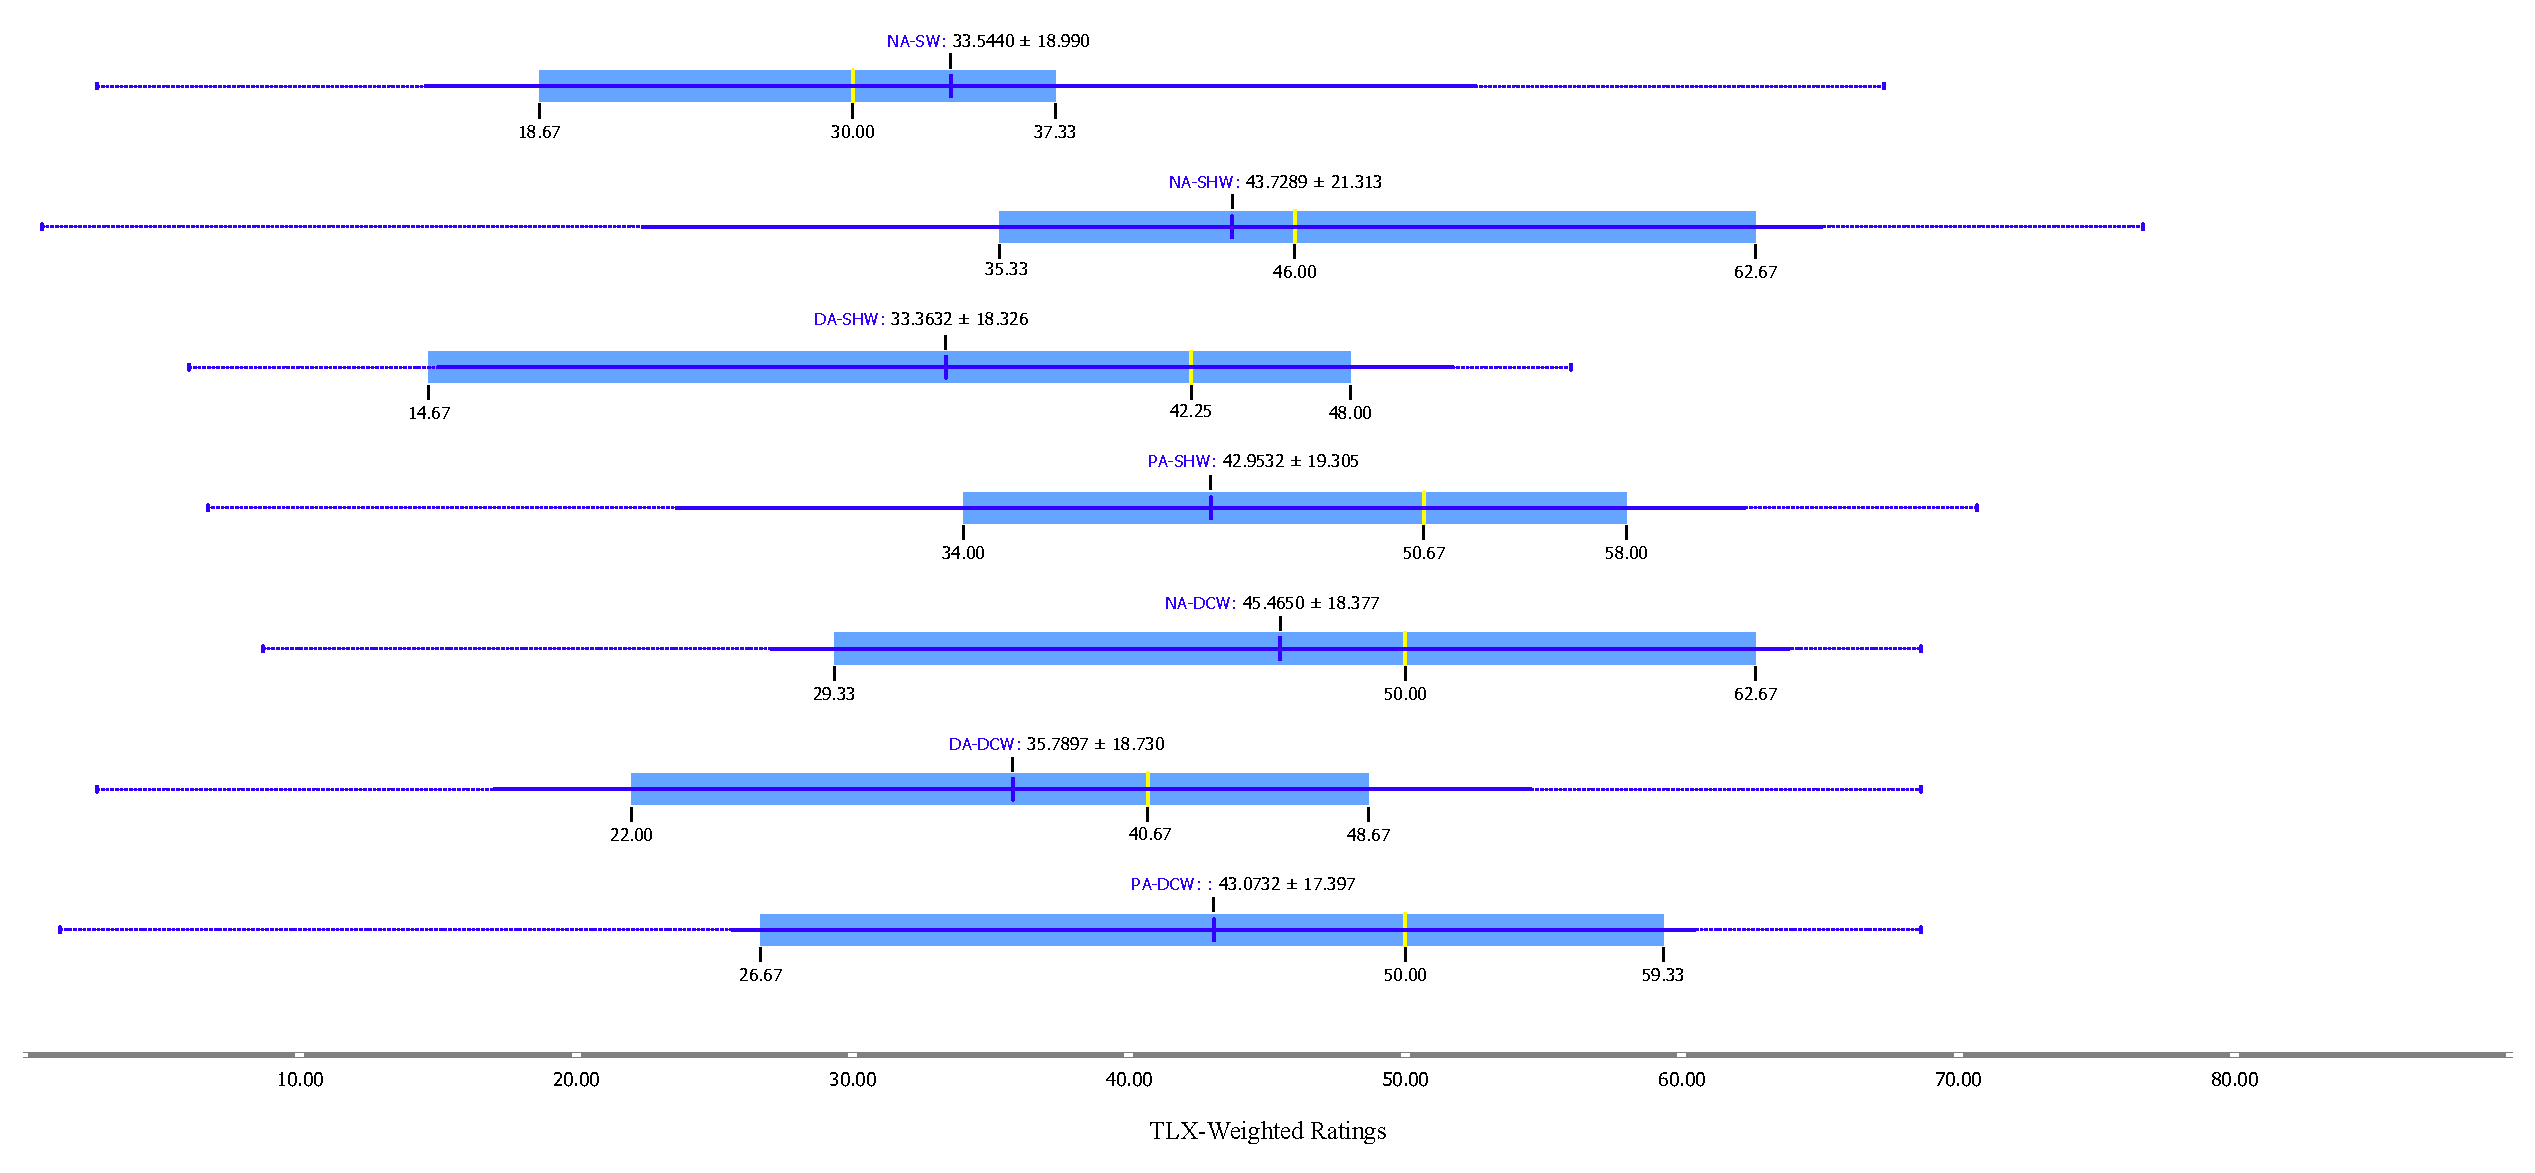
\includegraphics[width=\columnwidth]{images/tlx.pdf}
	\caption{Weighted ratings of the participants from NASA-TLX experiment wise.}
	\label{fig:weight}
\end{figure}

Using z-scores offers several advantages in our context. It provides standardisation, which is beneficial when dealing with varied interpretations of the NASA-TLX scale by different participants. This approach normalises the data, simplifying the categorization into distinct stress levels based on statistical criteria. 
In implementing this approach, we have set specific thresholds within the z-score distribution to categorise stress levels. These thresholds were carefully chosen based on a combination of empirical evidence and insights drawn from the literature. A z-score below 0 indicates a 'Not Stressed' state, scores between 0 and 1 correspond to a 'Slightly Stressed' condition, and scores above 1 are categorised as 'Stressed'. Therefore, the labels, which constitute a significant element of our model, were assigned by solely relying on subjective self-reports to categorise stress levels. The cross-validation of this methodology, which depends entirely on self-reports for stress labeling, with physiological signals and the broader implications and the applicability of this approach is detailed in later in sec........ For the present, this self-report-based system is the cornerstone of our labeling strategy.

\section{Classification -Stress Detection \gls{gptmg}}

In our stress detection model, we employed five machine learning algorithms with key settings for each:
\begin{itemize}
  \item \textbf{SVM (Support Vector Machine)}: Utilised via \texttt{sklearn.svm.SVC}, exploring various kernels such as linear, RBF, polynomial, and sigmoid. Key parameters included \texttt{C=1.0} and \texttt{gamma=0.1}.
  
  \item \textbf{Random Forest}: Implemented using \\ \texttt{sklearn.ensemble.RandomForestClassifier} with a focus on tuning parameters like the number of trees (n\_estimators=100). Features were scaled using \texttt{StandardScaler}.

  \item \textbf{Naive Bayes}: Employed using \texttt{GaussianNB} from \texttt{sklearn.naive\_bayes}, which is efficient for high-dimensional data.

  \item \textbf{K-Nearest Neighbors (KNN)}: Configured using \\ \texttt{sklearn.neighbors.KNeighborsClassifier} with the number of neighbors set to 10 and employing a suitable distance metric.

  \item \textbf{AdaBoost}: Applied through \texttt{sklearn.ensemble.AdaBoostClassifier}, optimizing the number of estimators and learning rate for performance enhancement.

  \item \textbf{Neural Network (MLP)}: Developed with \texttt{MLPClassifier} from \\ \texttt{sklearn.neural\_network}. The model had a single hidden layer with 100 neurons, used the ReLU activation function, and employed the Adam solver with \texttt{alpha=0.0008} and \texttt{max\_iter=200}.
\end{itemize}

These algorithms were chosen for their effectiveness and suitability in handling the complexities involved in stress classification. Each model was rigorously trained and evaluated using a 10-fold cross-validation approach to ensure robustness and reliability of the results.


\subsection*{Performance Assessment Metrics:}

To evaluate the performance of classification models, particularly in multi-class scenarios, we use a confusion matrix and several key metrics. A confusion matrix provides a detailed breakdown of a model's predictions against the actual values, offering insights into its performance across different classes.

\textbf{Confusion Matrix for a 3-Class Classification:}

A confusion matrix for a 3-class classification can be represented as follows:

\[
\begin{tabular}{|c|c|c|c|}
\hline
\textbf{Actual \textbackslash Predicted} & \textbf{Class 1} & \textbf{Class 2} & \textbf{Class 3} \\
\hline
\textbf{Class 1} & $\text{TP}_{1}$ & $\text{FP}_{12}$ & $\text{FP}_{13}$ \\
\hline
\textbf{Class 2} & $\text{FP}_{21}$ & $\text{TP}_{2}$ & $\text{FP}_{23}$ \\
\hline
\textbf{Class 3} & $\text{FP}_{31}$ & $\text{FP}_{32}$ & $\text{TP}_{3}$ \\
\hline
\end{tabular}
\]

In this matrix:
\begin{itemize}
    \item \textbf{TP (True Positive)}: Correct predictions of a specific class.
    \item \textbf{FP (False Positive)}: Incorrect predictions as a specific class, which actually belong to another class.
    \item \textbf{TN (True Negative)}: Correct predictions of instances not belonging to a specific class.
    \item \textbf{FN (False Negative)}: Incorrect predictions of instances as not belonging to a specific class, which actually do.
\end{itemize}

In this matrix, the diagonal elements ($\text{TP}_{1}$, $\text{TP}_{2}$, $\text{TP}_{3}$) represent the number of correct predictions for each class, while the off-diagonal elements indicate the misclassifications.

Using this matrix, the following metrics are calculated:

\begin{itemize}
    \item \textbf{Accuracy}: The proportion of correct predictions among the total number of cases examined.
    \[ \text{Accuracy} = \frac{\text{Sum of Diagonal Elements (TP)}}{\text{Total Number of Predictions}} \]

    \item \textbf{Precision} : The ratio of correct positive predictions to the total predicted as that class.
    \[ \text{Precision} = \frac{\text{TP}}{\text{TP} + \text{FP}} \]

    \item \textbf{Recall (Sensitivity)} : The proportion of actual positives of a class correctly identified.
    \[ \text{Recall} = \frac{\text{TP}}{\text{TP} + \text{FN}} \]

    \item \textbf{F1 Score} : The harmonic mean of precision and recall.
    \[ \text{F1 Score} = 2 \times \frac{\text{Precision} \times \text{Recall}}{\text{Precision} + \text{Recall}} \]
\end{itemize}

Another metric that is considered is the Area Under the Curve (AUC) metric of the ROC (Receiver Operating Characteristic) curve.  The ROC curve plots the true positive rate against the false positive rate at various threshold settings. AUC measures the entire  area underneath the ROC curve and provides an aggregate measure of the model's performance across all possible classification thresholds.

Accuracy provides an overall effectiveness of the model, while precision, recall, and F1 score offer class-specific performance insights, crucial in multi-class classification tasks.


\textbf{Cross-Validation Techniques}

We utilised two key cross-validation techniques to evaluate the performance and robustness of our machine learning models in stress detection: K-Fold Cross-Validation and Leave-One-Participant-Out (LOPO) Cross-Validation.

\begin{figure}[H]
  \centering
  % First image (shifted to the left)
  \hspace*{-2cm} % Adjust the value as needed to shift the image
  \begin{subfigure}[b]{0.50\columnwidth} % Adjust the width as needed
      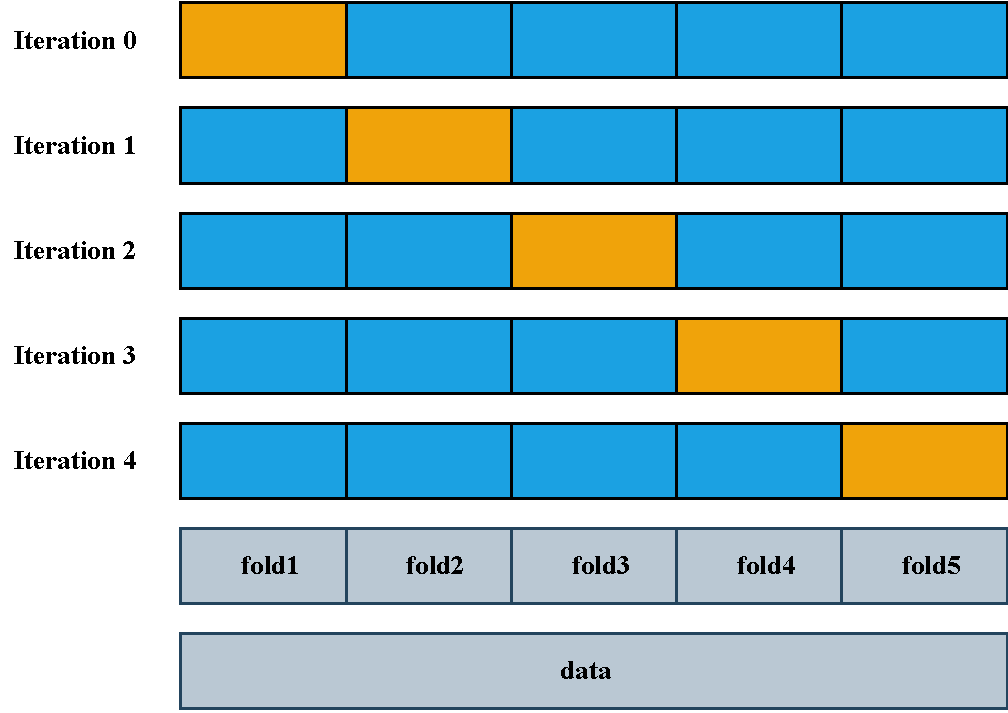
\includegraphics[width=\textwidth]{images/kfold.drawio.pdf}
      \caption{KFold}
      \label{fig:phone1}
  \end{subfigure}
  \hspace{0.05\columnwidth} % Adjust the horizontal space as needed
  % Second image
  \begin{subfigure}[b]{0.65\columnwidth}
      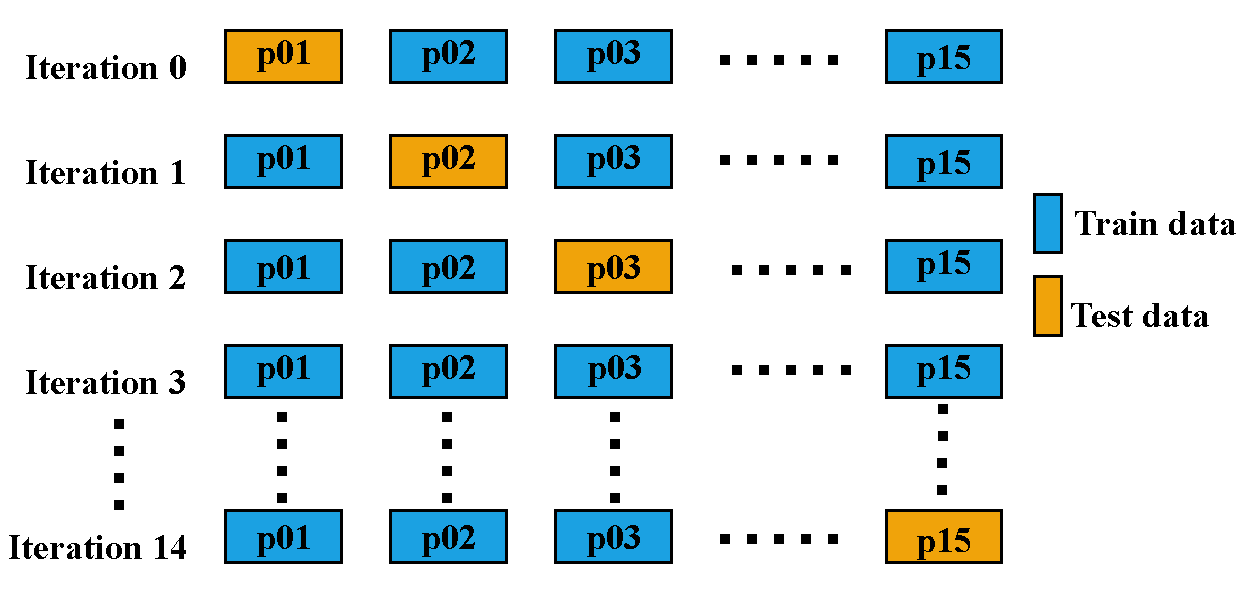
\includegraphics[width=\textwidth]{images/Lopo.drawio.pdf}
      \caption{LOPO}
      \label{fig:phone2}
  \end{subfigure}
  \caption{Cross Validation Techniques}
  \label{fig:CROSSVAL}
\end{figure}

\begin{itemize}
  \item \textbf{K-fold cross-validation:} \\
  K-Fold Cross-Validation is a standard method for assessing the efficacy of machine learning models. It involves dividing the entire dataset into 'K' equal-sized parts, or folds. The model is trained on 'K-1' of these folds, while the remaining fold is used for testing. This process is repeated 'K' times, each time with a different fold used as the test set, ensuring that each data point is used for both training and testing exactly once. The average performance across all 'K' iterations is used to estimate the model’s effectiveness.
  
  \item \textbf{Leave-One-Participant-Out (LOPO):} \\
  Leave-One-Participant-Out (LOPO) Cross Validation is particularly relevant for our study, which involves data collected from multiple participants. In this approach, the model is trained on data from all participants except one and then tested on the data from the left-out participant. This procedure is repeated for each participant, so in our case, with 15 participants, the process iterates 15 times. LOPO is especially beneficial in situations where participants undertake experiments in different orders. By training and testing the model on data from different participants, LOPO helps minimise potential biases that can arise due to variations in how participants respond to the experiment. This method allows for an unbiased assessment of the model's performance, as each subset of data (corresponding to each participant) is tested separately, and the results are aggregated to provide a comprehensive evaluation of the model’s effectiveness across the entire cohort.
\end{itemize}

These cross-validation techniques provide a thorough assessment of how well our model can generalise to new, unseen data, which is crucial for developing a reliable tool for stress detection.